\documentclass[border=5pt]{standalone}
\usepackage{tikz}
\usepackage{amsmath}
\usetikzlibrary{calc,intersections}
\usepackage{pgfplots}
\pgfplotsset{compat=1.16}
\usepgfplotslibrary{polar}
\begin{document}
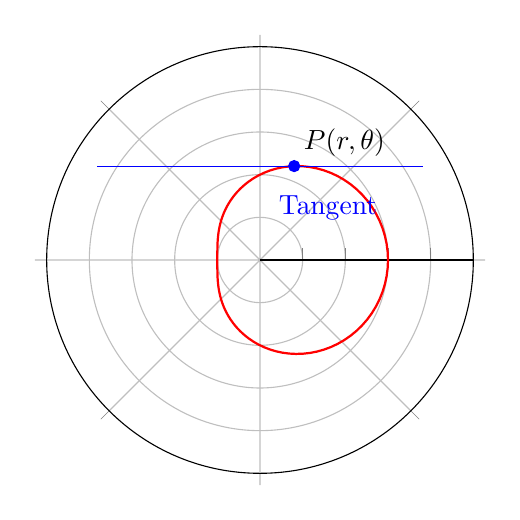
\begin{tikzpicture}

\begin{polaraxis}[
    width=7cm,
    height=7cm,
    grid=both,
    xmin=0, xmax=360,
    ymin=0, ymax=2.5,
    xtick={0,45,...,315},
    ytick={0.5,1,1.5,2},
    xticklabels={},
    yticklabels={},
]

    % Curve

    \addplot[red, thick, domain=0:360, samples=100] {1+0.5*cos(x)};



    % Point and tangent

    \pgfmathsetmacro{\angle}{70}

    \pgfmathsetmacro{\radius}{1+0.5*cos(\angle)}

    \pgfmathsetmacro{\slope}{(-0.5*sin(\angle)*sin(\angle) + \radius*cos(\angle))/(-0.5*sin(\angle)*cos(\angle) - \radius*sin(\angle))}



    \addplot[only marks, mark=*, blue, mark size=2pt] coordinates {(\angle,\radius)};



    % Tangent line (approximated)

    \pgfmathsetmacro{\xstart}{\radius*cos(\angle) - 0.7}

    \pgfmathsetmacro{\ystart}{\radius*sin(\angle) - 0.7*\slope}

    \pgfmathsetmacro{\xend}{\radius*cos(\angle) + 0.7}

    \pgfmathsetmacro{\yend}{\radius*sin(\angle) + 0.7*\slope}



    \addplot[blue, domain=30:150, samples=2] {\radius*sin(\angle)/sin(x)};



    % Labels

    \node[above right] at (axis cs:\angle,\radius) {$P(r,\theta)$};

    \node[blue, below right] at (axis cs:\angle+13,\radius-0.3) {Tangent};

\end{polaraxis}

\end{tikzpicture}
\end{document}
